\chapter{Принципы построения систем управления микроклиматом}

В аналогах систем управления теплицами можно выделить ряд подсистем, которые позволяют управлять микроклиматом теплицы.

Каждая из этих подсистем играет важную роль в обеспечении оптимальных условий для роста и развития растений в теплице. Автоматизация этих процессов позволяет сельскохозяйственным предприятиям повысить урожайность, снизить расходы на ресурсы и повысить эффективность производства. Вместе с тем, системы управления теплицами также способствуют сокращению человеческого вмешательства, что позволяет сельскохозяйственным работникам сосредоточиться на других важных задачах.

Ниже представлена примерная структурная схема подобных умных теплиц:

\begin{figure}[H]
    \centering
    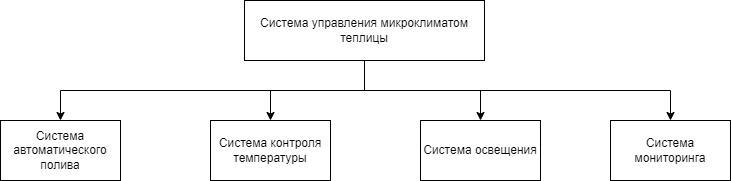
\includegraphics[scale=0.6]{images/system_schem.png}
    \caption{Структурная схема подсистем управления теплицей.}
    \label{fig:system_schem}
\end{figure}

Далее будет более подробно рассмотрена каждая из подсистем.

\section{Система автоматического полива}

Системы автоматического полива --- это удобный и эффективный способ поддерживать оптимальный уровень влажности почвы и обеспечивать растения водой без необходимости ручного полива. Существует множество различных видов систем автоматического полива, каждая из которых имеет свои достоинства и недостатки.

Одним из наиболее распространенных видов систем автоматического полива являются капельные системы. Они основаны на том, что вода подается к растениям маленькими каплями через тонкие трубки, расположенные непосредственно у корней растений. Капельные системы позволяют сберегать воду, поскольку вода подается непосредственно к растениям, минуя неиспользуемые участки почвы. Кроме того, капельные системы помогают избежать разбрызгивания воды, что может быть особенно полезно для тепличных культур~\cite{Watering,Watering2}.

Другой распространенный вид систем автоматического полива --- это системы распыления. Вода подается к растениям в виде тумана через дождеватели или специальные распылители. Системы распыления имеют преимущество в том, что они позволяют равномерно распределять воду по всей территории участка, а также удобны для полива крупнолистных и больших растений.

Также существуют системы автоматического полива, основанные на гидропонике, о которой было написано ранее.

Некоторые системы автоматического полива оснащены датчиками влажности почвы, которые позволяют определить уровень влажности в почве и подавать воду только в том случае, если почва стала слишком сухой. Это помогает сократить расход воды и уменьшить нагрузку на систему автоматического полива.

Несмотря на множество преимуществ, системы автоматического полива также имеют свои недостатки:

\begin{enumerate}
    \item ошибки в работе. Системы автоматического полива могут не всегда правильно распознавать необходимость полива и выполнять его в ненужное время или наоборот, не выполнять полив в нужное время;
    \item риск переувлажнения почвы. Некоторые системы автоматического полива могут приводить к избыточному поливу и переувлажнению почвы, что может негативно сказаться на росте растений и привести к их гибели;
    \item необходимость подключения к источнику электропитания. Системы автоматического полива нуждаются в постоянном подключении к источнику электропитания, что может быть неудобно в случае отсутствия возможности подключения или ограниченных ресурсов;
    \item зависимость от погодных условий. Некоторые системы автоматического полива могут быть неэффективными в случае экстремальных погодных условий, таких как длительная засуха или сильные дожди.
\end{enumerate}

\section{Система контроля  температуры}

Система контроля температуры теплицы --- это комплекс различных элементов, направленных на поддержание оптимального режима температуры внутри теплицы для растений~\cite{Temperature}.

Основными элементами системы контроля температуры теплицы являются:

\begin{enumerate}
    \item термостат: устройство, которое автоматически регулирует температуру внутри теплицы. Термостат может быть механическим, электронным или программным, в зависимости от конкретной модели;
    \item обогреватель: устройство, которое используется для поддержания оптимальной температуры внутри теплицы в зимнее время или при холодной погоде;
    \item окна вентиляции: окна или заслонки, которые открываются автоматически для регулирования температуры в теплице при необходимости;
    \item вентиляторы: устройства, которые могут использоваться для циркуляции воздуха и снижения температуры в теплице;
    \item датчики температуры: устройства, которые используются для контроля температуры внутри теплицы и передачи данных в систему управления.
\end{enumerate}

Система контроля температуры теплицы имеет следующие достоинства:

\begin{enumerate}
    \item автоматическое поддержание оптимальной температуры для растений, что способствует росту и повышает урожайность;
    \item экономия времени и сил на ручное регулирование температуры в теплице;
    \item снижение риска перегрева или переохлаждения растений, что может привести к их гибели.
\end{enumerate}

Однако, система контроля температуры теплицы также имеет некоторые недостатки:

\begin{enumerate}
    \item в случае сбоя в системе может произойти сильное изменение температуры в теплице, что может негативно повлиять на рост и развитие растений;
    \item необходимость регулярной проверки и обслуживания системы для ее бесперебойной работы.
\end{enumerate}

\section{Система освещения}

Система освещения в умной теплице --- это важный компонент, который обеспечивает растения необходимым количеством света в течение дня и дополнительной подсветкой в период недостаточной освещенности. Система освещения в умной теплице может быть автоматизирована и интегрирована в систему управления климатом, что позволяет оптимизировать режим освещения в зависимости от требований растений и экономить электроэнергию~\cite{Light}.

Основные компоненты системы освещения в умной теплице:

\begin{enumerate}
    \item лампы (LED или люминесцентные) - обеспечивают освещение в теплице;
    \item датчики освещенности - измеряют уровень освещенности в теплице;
    \item контроллер освещения - автоматически управляет работой ламп, основываясь на показаниях датчиков и заданных параметрах.
\end{enumerate}

Достоинства системы освещения в умной теплице:

\begin{enumerate}
    \item автоматизация работы системы освещения, что позволяет экономить время и ресурсы;
    \item оптимизация режима освещения в зависимости от требований растений, что позволяет повысить урожайность и качество продукции;
    \item экономия электроэнергии за счет оптимизации работы системы освещения.
\end{enumerate}

Недостатки системы освещения в умной теплице:

\begin{enumerate}
    \item риски сбоев и отказов в работе системы освещения, что может негативно сказаться на росте растений;
    \item необходимость правильного подбора ламп и параметров освещения для каждого вида растений.
\end{enumerate}

\section{Система мониторинга}

Система мониторинга в умной теплице предназначена для наблюдения и контроля за условиями внутри теплицы, такими как температура, влажность, освещенность, уровень $CO_2$ и другие параметры, влияющие на рост и развитие растений.

Основными элементами системы мониторинга являются датчики, которые устанавливаются внутри теплицы и считывают данные об условиях окружающей среды. Эти данные затем передаются на управляющий блок, который обрабатывает информацию и, если необходимо, производит регулировку условий внутри теплицы~\cite{Monitoring}.

Достоинства системы мониторинга:

\begin{enumerate}
    \item позволяет контролировать и регулировать условия внутри теплицы, что положительно сказывается на росте и развитии растений;
    \item помогает предотвратить опасные для растений условия, такие как перегрев или переохлаждение;
    \item система мониторинга может быть настроена на автоматическое управление другими системами теплицы, такими как системы полива или освещения.
\end{enumerate}

Недостатки системы мониторинга в умной теплице:

\begin{enumerate}
    \item высокая стоимость установки и обслуживания;
    \item сложность установки и настройки системы;
    \item необходимость постоянного мониторинга и обслуживания системы, чтобы избежать ее сбоев.
\end{enumerate}

Система мониторинга является важным компонентом умной теплицы, который помогает обеспечить оптимальные условия для роста и развития растений и улучшить их урожайность. Однако, перед установкой системы мониторинга необходимо тщательно оценить ее достоинства и недостатки и принять решение, насколько она подходит для конкретных потребностей и условий внутри теплицы.

Для достижения более высокой степени автоматизации и контроля микроклимата, все эти системы должны работать в синхронизации и объединяться в единую комплексную систему, которая будет оптимизировать их функционирование.

Исходя из представленных систем автоматического регулирования, можно выделить ключевые задачи, которые они выполняют:

\begin{enumerate}
    \item регулирование температуры воздуха;
    \item управление системой полива;
    \item контроль и управление осветительными устройствами.
\end{enumerate}

Поддержка заданных климатических параметров является неотъемлемой составляющей для обеспечения эффективного и стабильного функционирования системы микроклимата. Каждое растение имеет определенные требования к температуре, влажности, освещенности и другим климатическим условиям, которые оптимизируют и поддерживают его здоровье и рост. Если климатические параметры выходят за пределы заданных значений, это может негативно сказаться на растениях, привести к заболеваниям, повреждениям или даже гибели. Поэтому системы микроклимата разрабатываются с целью обеспечить точное и надежное контролирование климата внутри теплицы или иного пространства, где происходит выращивание растений. Именно поддержка заданных климатических параметров является ключевым фактором для успешного и продуктивного выращивания растений в управляемой среде и обеспечивает оптимальные условия для их здоровья и процветания.